\begin{frame}{Les trois dispositifs connus}
    \begin{itemize}
        \item \textbf{les blogues} = premiers à accueillir des récits de soi, à travers la pratique du journal.
        \item \textbf{les vlogues} = déclinaison du blogue, un peu plus tardive, qui va consacrer la figure de l'amateur, avec le développement de YouTube.
        \item \textbf{les profils numériques} = complexité supplémentaire à la réflexion sur l'identité numérique, en abordant la question de nos données, notamment personnelles.
    \end{itemize}
\end{frame}

\begin{frame}{Les blogues et l'auto-blographie}
    \begin{itemize}
        \item Mot-valise issu de web-log (journal Web)
        \item Premières formes d'expression de soi sur le Web
        \item Remédiation du journal 
        \item Succès à partir des années 2000 (MySpace, Skyblogs, etc...)
    \end{itemize}
    
\end{frame}

\begin{frame}{Écrire pendant le web 1.0 (ou web statique)}
    \begin{block}{Les journaux du premier Web}
        \begin{figure}
    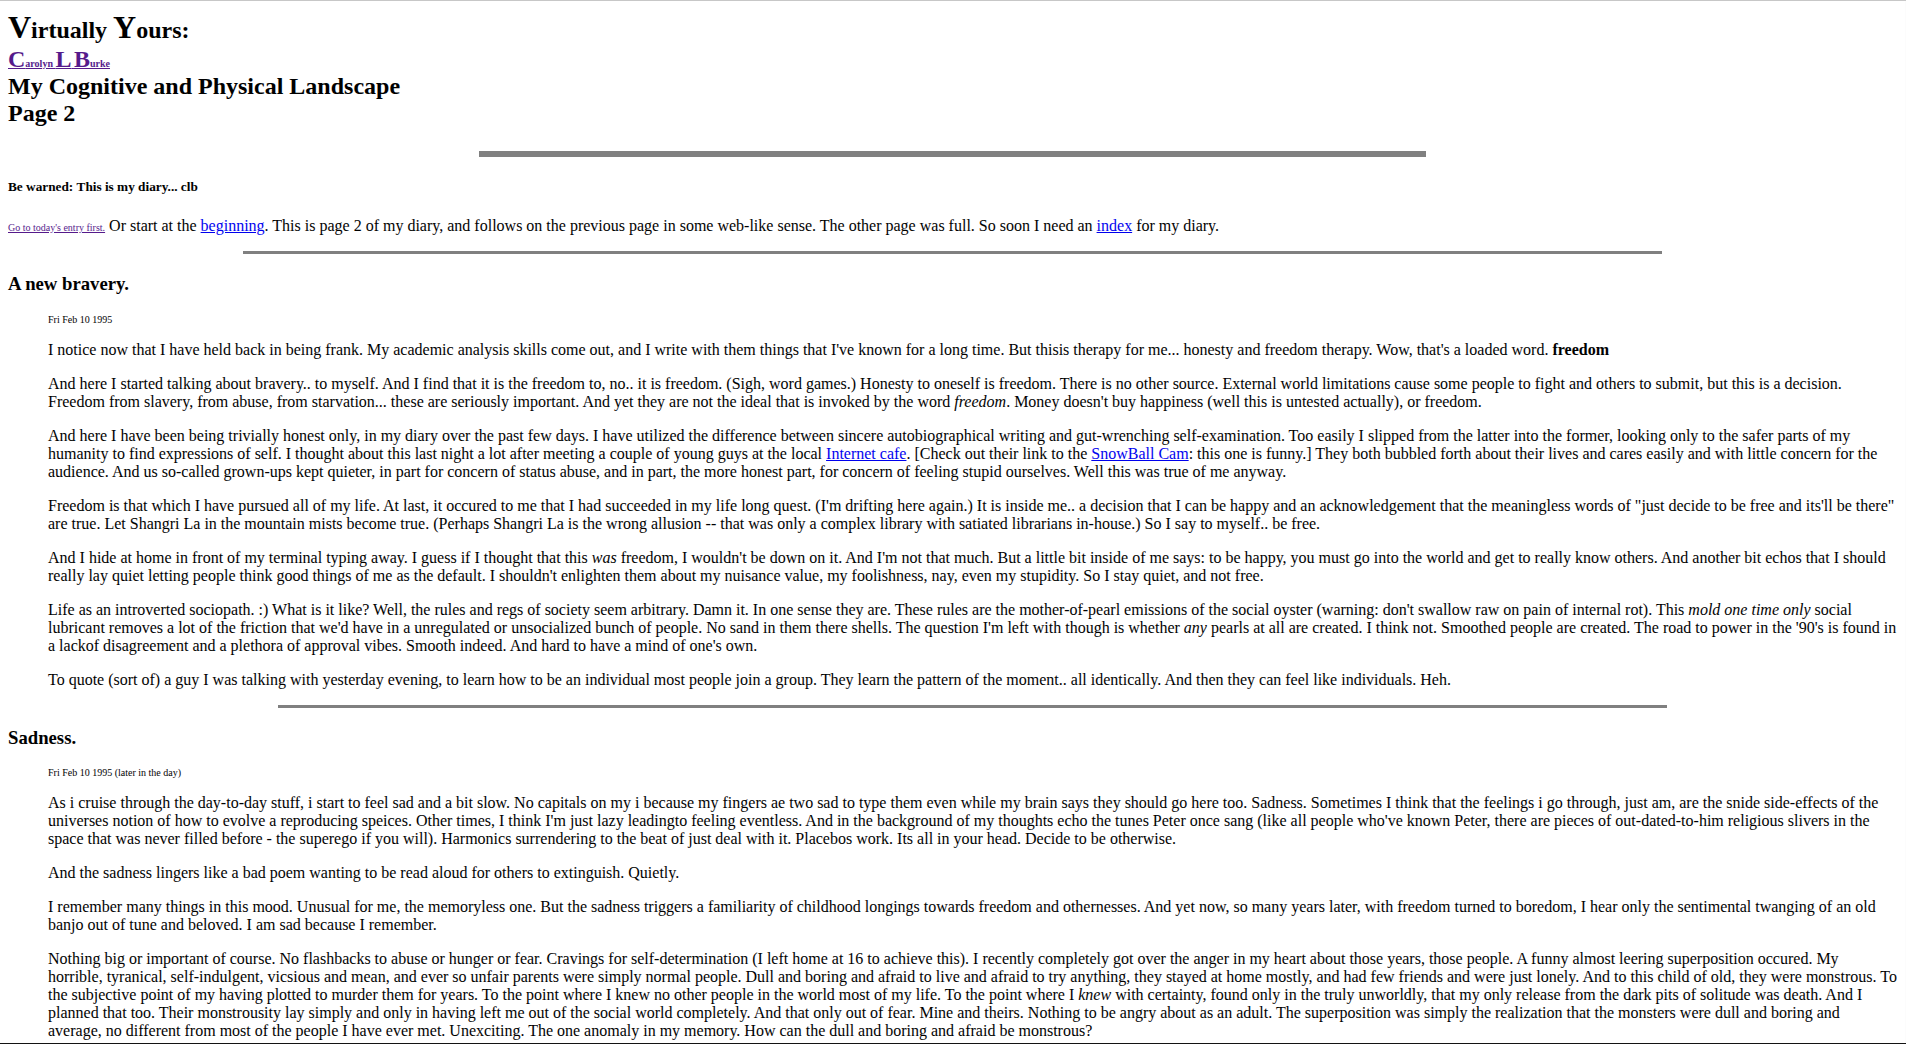
\includegraphics[width=\textwidth]{Images/Carolyn_burke.png}
        \end{figure}
    
    \end{block}
    
\end{frame}
\begin{frame}{Les blogues du Web 2.0 (ou web social années 2000)}
    \begin{itemize}
        \item Essor de la contribution en ligne
        \item Paradigme de la participation
    \end{itemize}
    \centering
    \begin{figure}
        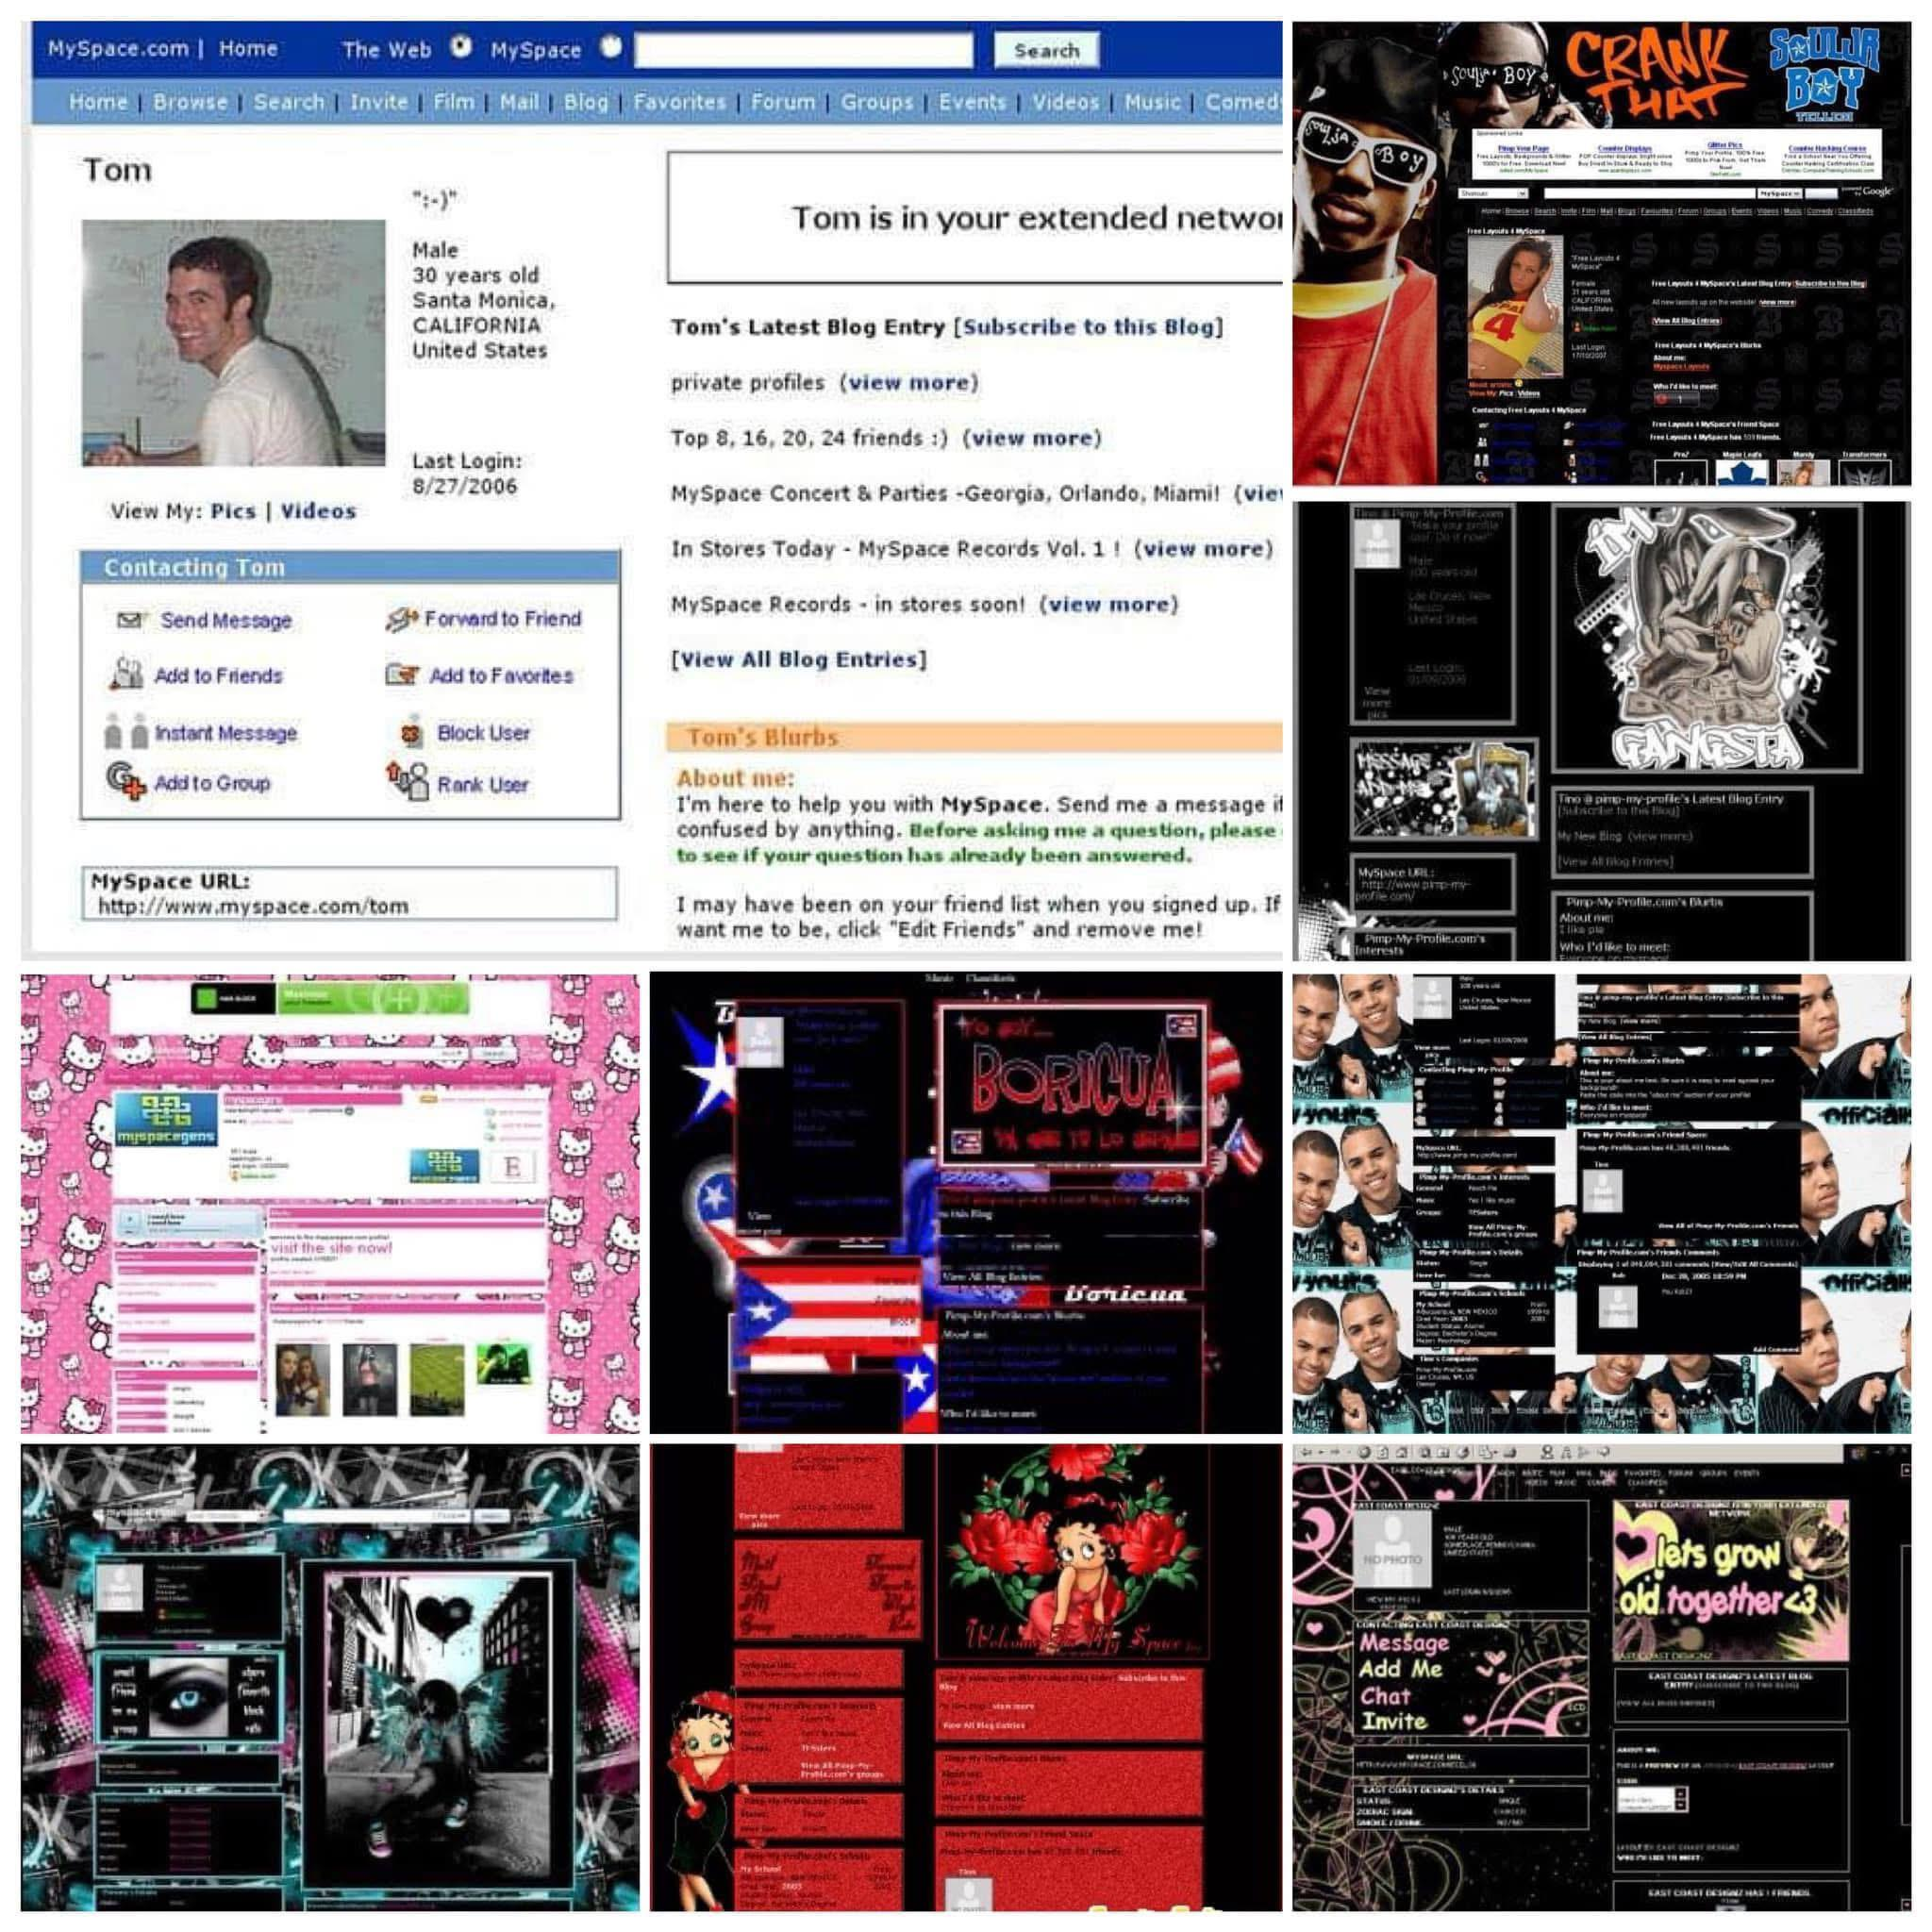
\includegraphics[width=.4\textwidth]{Images/myspace.jpeg}
        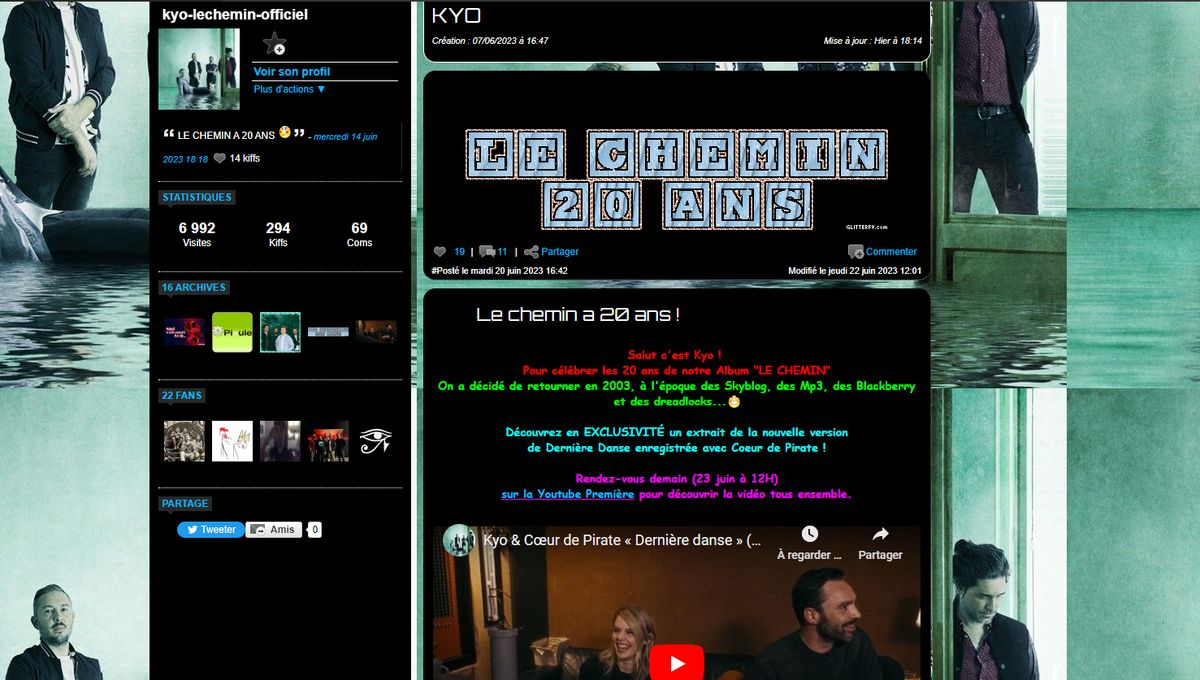
\includegraphics[width=.5\textwidth]{Images/skyblog.jpeg}
    \end{figure}
\end{frame}

\begin{frame}{Le temps des vlogues : les journaux filmés, ou l'exploration plurimédiatique du web}
\begin{columns}
    % Colonne de gauche : Texte
        \begin{column}{0.4\textwidth}
            
    \begin{itemize}
        \item Sortir le journal de l'écrit
        \item Publication sur des plateformes spécialisées
        \item Développement d'une nouvelle intimité, à travers des dispositifs tels que le "live streaming".
    \end{itemize}
        \end{column}

        % Colonne de droite : Image
        \begin{column}{0.5\textwidth}
            \centering
            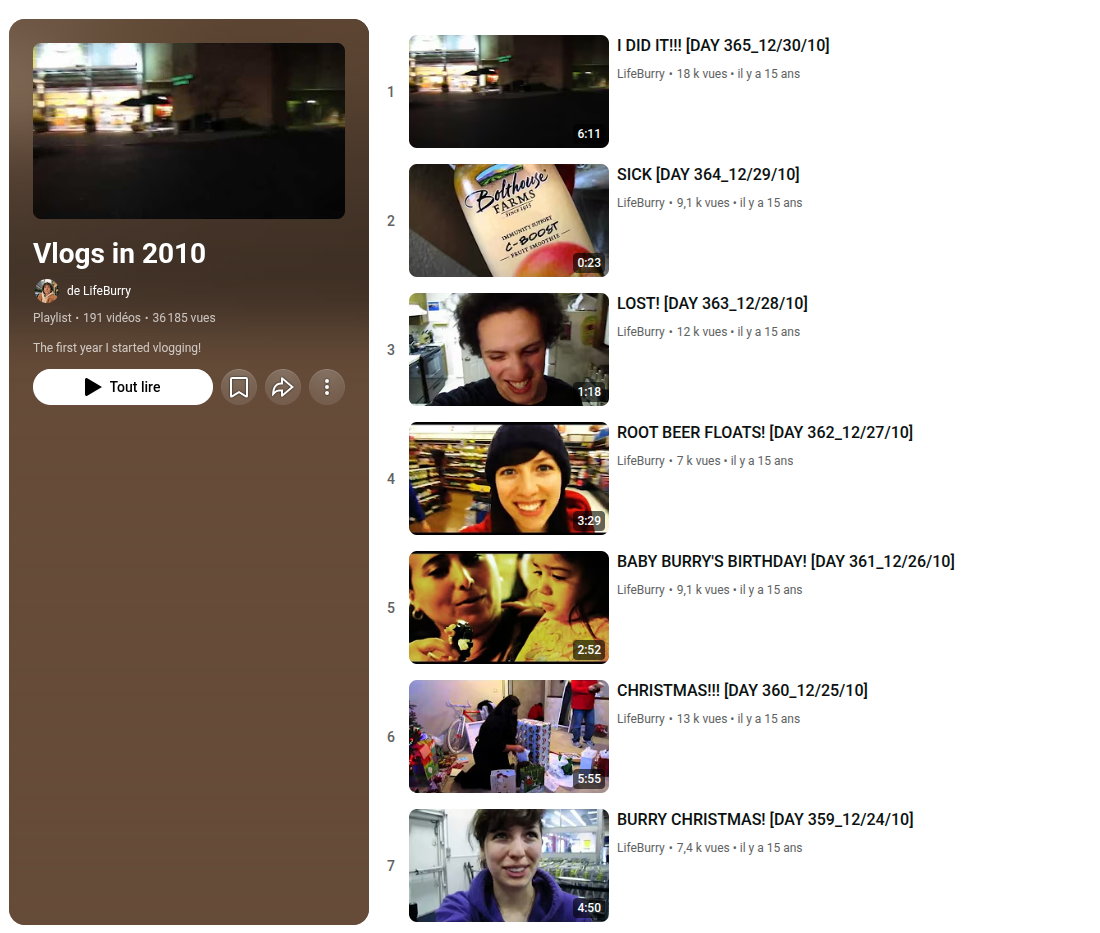
\includegraphics[width=.9\textwidth]{Images/vlogs.png}
        \end{column}
    \end{columns}
    
\end{frame}

\begin{frame}{Le temps des vlogues : les journaux filmés, ou l'exploration plurimédiatique du web}

    \begin{figure}
        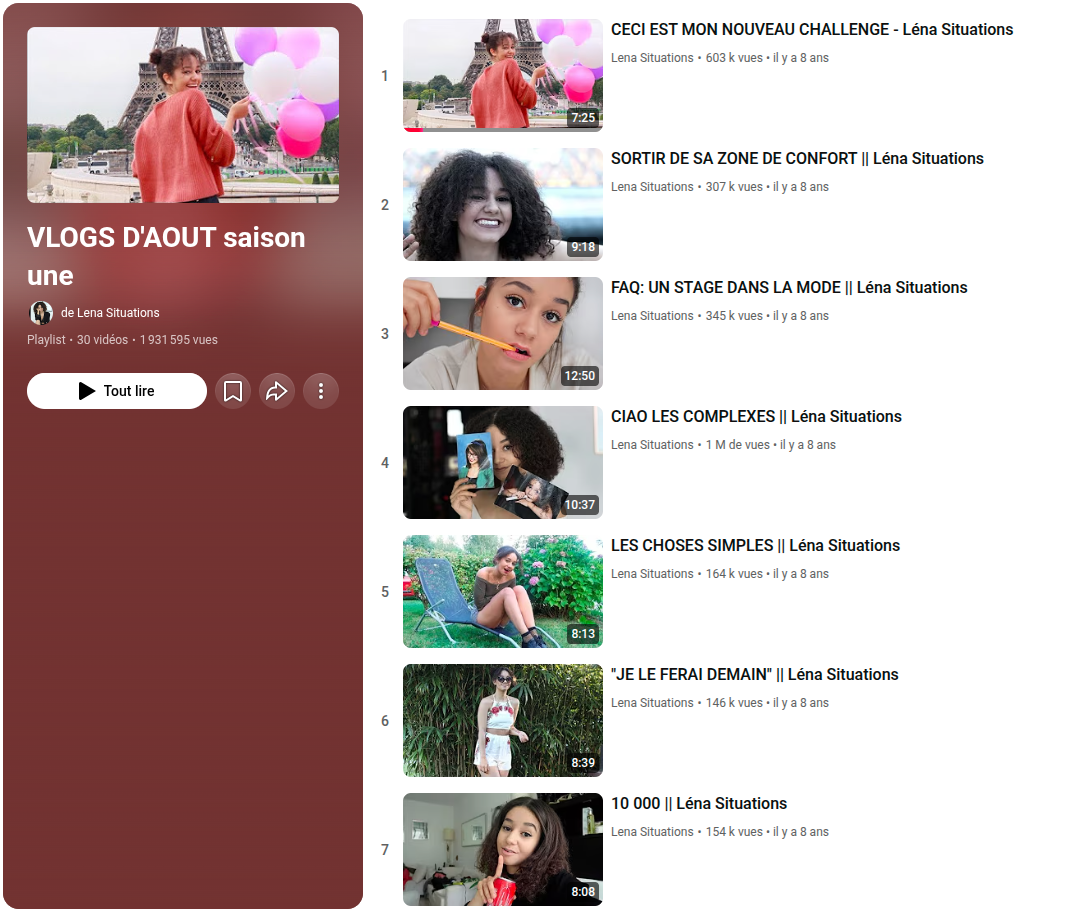
\includegraphics[width=.6\textwidth]{Images/lena_situation_vlog.png}
    \end{figure}
    
\end{frame}